\documentclass{examnotes}

\header{STA2603 Distribution Theory II}
%%%%%%%%%%%%%%%%%%%%%%%%%%%%%%%%%%%%%%%
\begin{document}

\h{STA2603 Distribution Theory II}

{\red{Always specify the domain of the function!}} \hfill  {\red{Always specify the parameters when identifying the distribution!}}


\h{Study Unit 2}

Frequency Function (discreet) = density function (continuous).
Distribution functions is CDF.

\h{Discreet Random Variables}

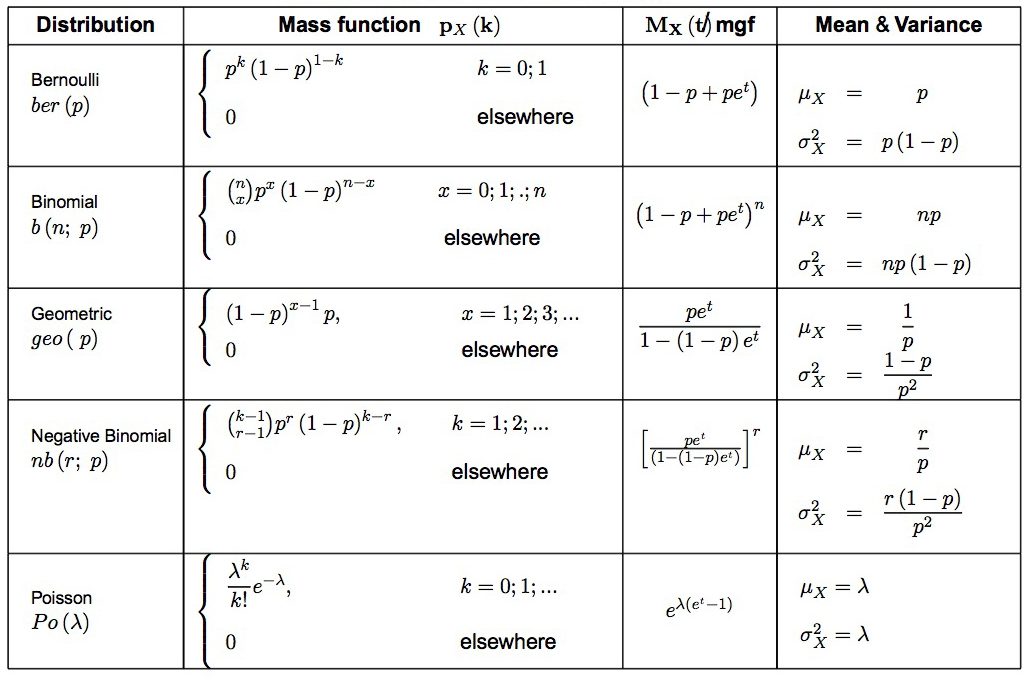
\includegraphics[scale=0.5]{./img/disscreet.jpg}

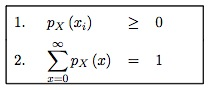
\includegraphics[scale=0.8]{./img/2dis.jpg}

\sh{Bernoulli Random Variables}

\vspace{6pt}

Indicator random variable \mymath{I_A(\omega)=\begin{cases} 1 & \omega \in A\\
0 & \text{otherwise}
\end{cases}
} %\mymath

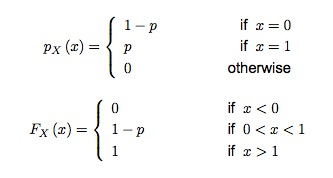
\includegraphics[scale=0.6]{./img/2ber.jpg}


\sh{Binomial Distribution}

The sum of independent Bernoulli variables is a binomial random variable. 

To prove binomial probabilities sums to 1. Use finite binomial series expansion:
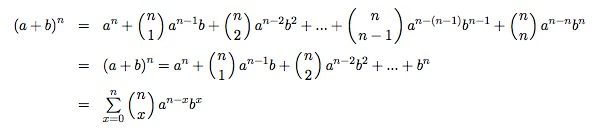
\includegraphics[scale=0.7]{./img/2ber2.jpg}
\vspace{-10pt}

and therefore it is a series expansion of $[(1-p)+p]^n$

\vspace{6pt}
\sh{Geometric Distribution}

To prove that geometric distribution sums to 1, use Taylor series at x=0
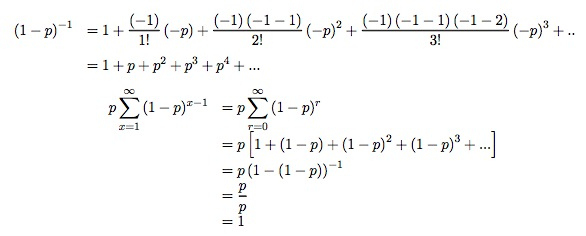
\includegraphics[scale=0.7]{./img/2geo.jpg}

\clearpage
\sh{Negative Binomial Distribution}

A negative binomial random variable can be expressed as the sum of \emph{r} independent geometric variables.

{\sh{Hypergeometric distribution}
\vspace{6pt}

\mymath{pX(x)=\begin{cases} \displaystyle\frac{\binom{r}{x}\binom{n-r}{m-x}}{\binom{n}{m}} & \text{if }x=0,1,2,\dots.n\\
0 & \text{otherwise}
\end{cases}
} %\mymath

\sh{Poisson Distribution}

To show it is a frequency function: 

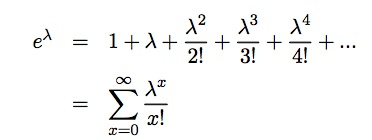
\includegraphics[scale=0.7]{./img/2poi1.jpg}

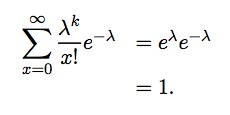
\includegraphics[scale=0.7]{./img/2poi2.jpg}

Poisson distribution can be used to approximate binomial distribution, if \emph{n} is large and \emph{p} is small.

\h{Continuous Random Variables}

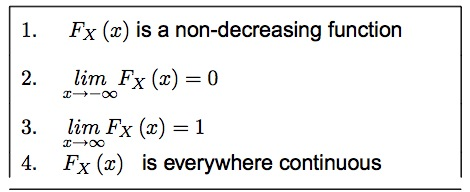
\includegraphics[scale=0.7]{./img/2con1.jpg}

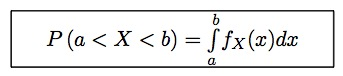
\includegraphics[scale=0.7]{./img/2con2.jpg}

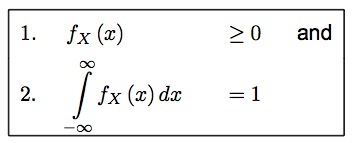
\includegraphics[scale=0.7]{./img/2con3.jpg}

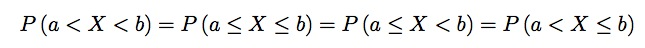
\includegraphics[scale=0.7]{./img/2con4.jpg}

The $p$th quantile: $F(x_p)=p$ \quad or $P(X\le x_p)=p$ \quad and $x_p=F^{-1}(p)$

\sh{Exponential Density}

\sh{Gamma Density}

Gamma function $\Gamma(a)=\displaystyle\int_0^\infty{x^{a-1}e^{-x}}$ \quad Properties $\Gamma(\alpha+1)=\alpha\Gamma(\alpha)$ \quad $\Gamma(\frac{1}{2})=\sqrt{\pi}$
\quad $c^n\Gamma(n)=\displaystyle\int_0^\infty{x^{n-1}e^{-\displaystyle\frac{x}{c}}}$

$\Gamma(2) = 1$ \vspace{6pt}

If $\alpha=1$ then it becomes exponential density


If $\lambda=1$ then it is a one parameter gamma density

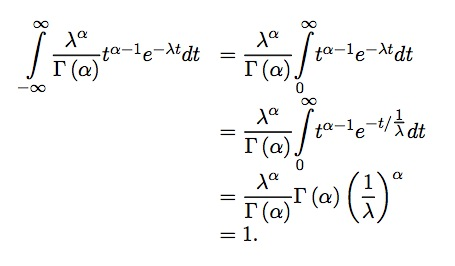
\includegraphics[scale=0.4]{./img/2gam.jpg}


\sh{Normal (Gaussian) distribution}

\sh{Beta Density}

Beta function: $B(m,n)=\displaystyle\int_0^1{x^{m-1}(1-x)^{n-1}dx}$ \quad or $B(m,n)=\displaystyle\int_0^\infty{\frac{x^{n-1}}{(1+x)^{m+n}}dx}$

To prove density function:

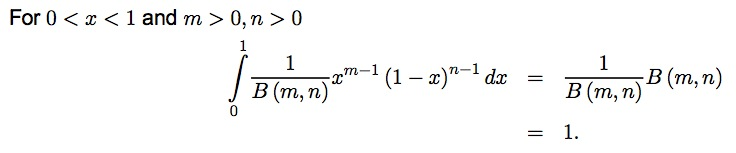
\includegraphics[scale=0.4]{./img/2bet2.jpg}

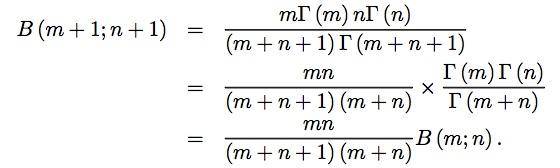
\includegraphics[scale=0.4]{./img/2bet3.jpg}

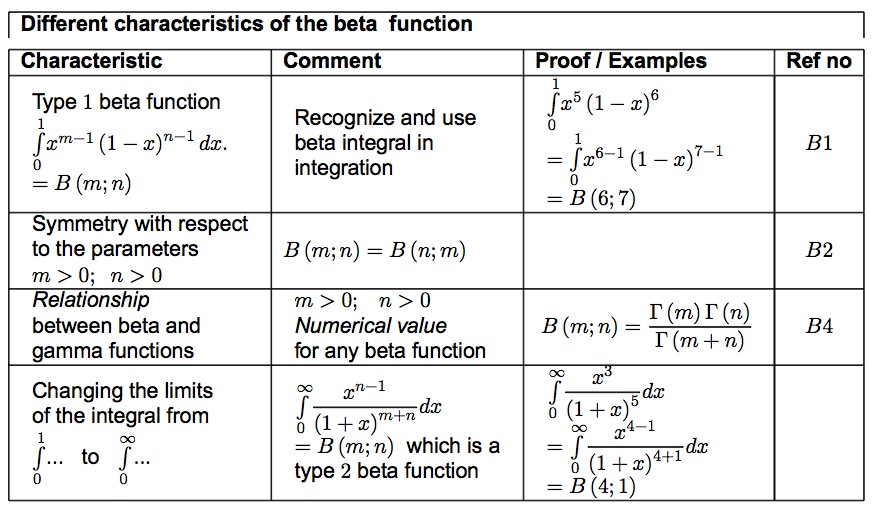
\includegraphics[scale=0.5]{./img/2bet1.jpg}

\h{Functions of random Variables}

Standard normal CDF $= \Phi(X)$ \quad Standard normal density $= \varphi(X)$

{\bf Proposition A:}
if $X\mytilde N(\mu,\sigma^2)$ and $Y=aX+b$, then $Y\mytilde N(a\mu+b,a^2\sigma^2)$

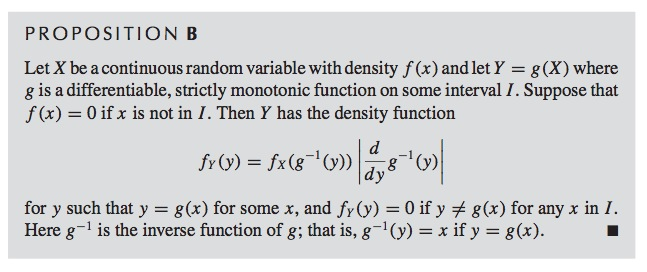
\includegraphics[scale=0.6]{./img/2fun1.jpg}

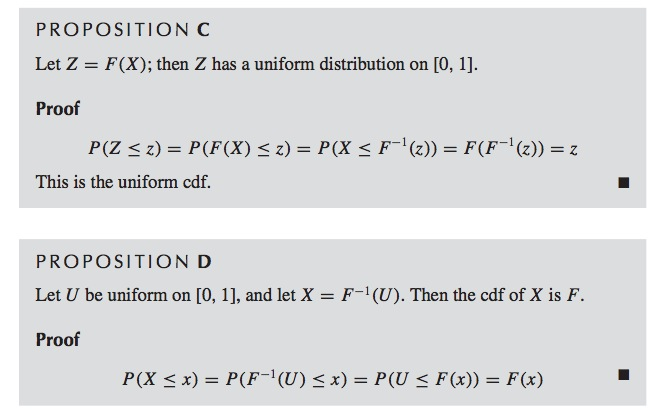
\includegraphics[scale=0.6]{./img/2fun2.jpg}

$[N(0,1)]^2\mytilde \chi^2_1$

Weibull density: $\displaystyle\frac{\beta}{\alpha^\beta}x^{\beta-1}e^{-\left(\displaystyle\frac{x}{\alpha}\right)^\beta}$

%%%%%%%%%%%%%%%%%%%%%%%%%%%%%%%%%%%%%%%
\h{Study Unit 3: Joint Distributions}

\sh{Discreet Random Variables}

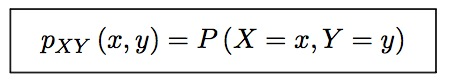
\includegraphics[scale=0.4]{./img/3jd1.jpg}

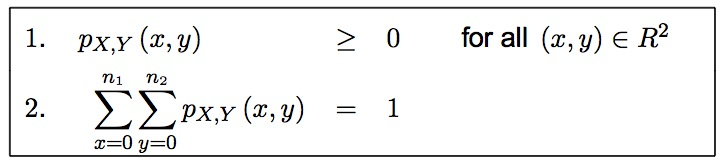
\includegraphics[scale=0.4]{./img/3jd2.jpg}

\sh{Continuous Random Variables}

Marginal density.

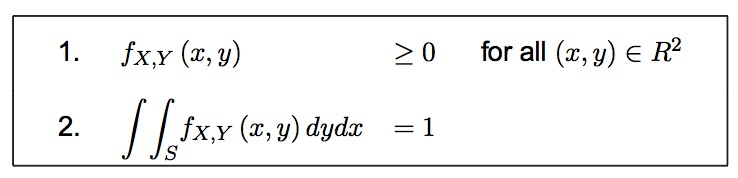
\includegraphics[scale=0.4]{./img/3con1.jpg}                                         

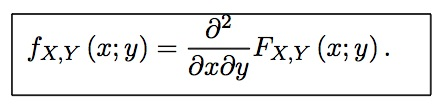
\includegraphics[scale=0.4]{./img/3con2.jpg}                                         

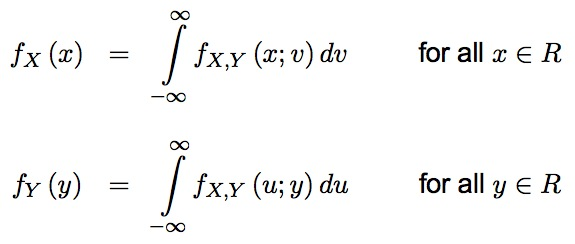
\includegraphics[scale=0.4]{./img/3con3.jpg}                                         

\red{Marginals sum to 1}

Joint cumulative distribution.

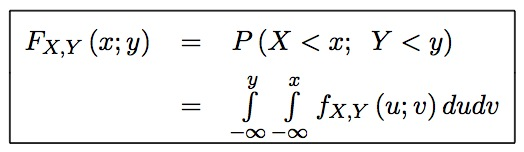
\includegraphics[scale=0.4]{./img/3con4.jpg}                                         


\sh{Independent Random variables}

Independent if $F(x,y)=F_X(x)F_Y(y)$

Two discreet random variables will be independent if th their joint mass function factors.

\sh{Conditional Distributions}

Discreet:

The law of total probability. $p_X(x)=\displaystyle\sum_y{p_{X|Y}(x|y)p_Y(y)}$

Continuous:

The law of total probability. $f_Y(y)=*\int_{-\infty}^\infty{f_{Y|X}(y|x)f_X(x)\,dx}$

















\end{document}
